\subsubsection{\stid{3.13} CLOVER Sub-project PEEKS} \label{subsubsect:peeks}
\paragraph{Overview} 
The PEEKS subproject is a focused team effort to advance the capabilities of the
ECP software stack in terms of communication-avoiding Krylov solvers and
advanced preconditioning techniques featuring fine-grained parallelism.
Previously developed techniques that are available as prototype codes -- as
well as novel algorithm developments -- are turned into production-quality 
implementations and integrated into the ECP software ecosystem 
as part of the Trilinos~\footnote{\url{https://trilinos.org/}} and the  
Ginkgo~\footnote{\url{https://github.com/ginkgo-project/ginkgo}} software 
stacks. 
%With the PEEKS project focus being on algorithm development an software design 
%and leading developers of the Trilinos and Ginkgo software packages being 
%involved in the PEEKS project, a strong focus is on software interoperability 
%and software sustainability. In consequence, there exists a strong link to the 
%other ECP math libraries and the xSDK4ECP project coordinating the ECP 
%mathematical library interoperability efforts. All technology developed in 
%PEEKS is available and disseminated via the xSDK software stack.


\paragraph{Key  Challenges}
Developing preconditioned iterative solvers for the US flagship supercomputers 
deployed in ECP, we acknowledge three major challenges coming from the hardware 
architecture:
\begin{enumerate}
\item 
Fine-grained parallelism in a single node that has to be exploited efficiently 
by the iterative solver and the preconditioner.
\item
Rising communication and synchronization cost.
\item
Computational power growing much faster than memory power, resulting on 
increased pressure on the bandwidth of all cache/memory levels.
\item 
Low-precision special function units like Tensor cores that are increasingly 
adopted by hardware architectures require sophisticated numerical schemes to be 
useful for general purpose scientific computing.
\end{enumerate}

All challenges require the redesign of existing iterative solvers with respect 
to higher parallelism, % within all building blocks
a reduced number of 
communication and synchronization points, favoring computations over 
communication, and adopting multiprecision algorithms for efficient hardware 
utilization. 
In the last few decades, numerous efforts 
have investigated the potential of communication-avoiding (CA) and pipelined 
Krylov solvers~\cite{yamazakiipdps2014,Cornelis2018TheCC},
% ; however, the implementations usually remained in prototype status and rarely made it into production code. 
% Similarly, significant effort was put into developing 
as well as new preconditioning 
techniques that allow for the efficient parallelization of the preconditioner 
setup and the preconditioner 
application~\cite{chowisc2015,anzteuropa2015,ANZT20181}. 
However, most implementations were experimental and rarely adopted by application 
code.
Also the concept of accelerating iterative methods by using lower precision 
formats for parts of the computations or memory access was extensively 
investigated in literature~\cite{carson1,carson2,doi:10.1002/cpe.4460}, 
while production-ready implementations are still scarce.

%In the PEEKS project we address the challenge of turning prototype 
%implementations into production-ready functionality by improving robustness 
%and 
%safeguarding against numerical breakdown, developing application- and 
%architecture-specific optimizations, and integrating into ECP application 
%projects and into a sustainable and extensible mathematical software stack.

\paragraph{Solution Strategy}

The primary thrusts of the PEEKS project are:
\begin{enumerate}
    \item \textbf{Architecture-portable software design:}
	In the Ginkgo C++ software, we design and develop a next-generation 
	sparse linear algebra library able to run on multi- and manycore 
	architectures. The library design decouples
	algorithm implementations from hardware-specific kernel implementations, 
	thereby allowing extensibility as well as 
	architecture-specific kernel optimization. 
   \item \textbf{Sustainability efforts:}
	The Ginkgo software development cycle adheres the Better Scientific 
	Software (BSSw) design principles~\cite{betterscientificsoftware} that 
	ensure production-quality code by featuring unit testing, automated 
	configuration and installation, Doxygen code documentation, as well as a 
	continuous integration and continuous benchmarking 
	framework~\cite{pasc_anzt}. Ginkgo is an 
	open source effort licensed under BSD 3-clause and ships with the latest 
	version of the xSDK package (v.0.5.0). 
   \item \textbf{Pipelined and CA Krylov methods:} 
    We realize pipelined and 
	communication-avoiding Krylov methods in production-quality code, and 
	we are actively collaborating with the ECP ExaWind project to integrate 
        our new features into their application~\cite{Yamazaki-lowsynch}. 
	\item \textbf{ParILUT -- A parallel threshold ILU:}  We are spearheading 
	the manycore-parallel computation of threshold-based 
	incomplete factorization preconditioners~\cite{sisc_anzt,ipdps_anzt}. 
	\item \textbf{Adaptive precision block-Jacobi:}  We realized a 
	production-ready block-Jacobi preconditioner that reduces the runtime by 
	carefully selecting the storage format of the distinct block inverses 
	without impacting the preconditioner quality~\cite{toms_anzt}. 
   \item \textbf{Software-defined events (SDE):}  We team up with the ECP 
    Exa-PAPI project to design and realize an ecosystem for software-defined 
    events. The idea is to provide 
% application scientists with 
    easy access 
    to library-, domain- and solver-specific metrics via the PAPI interface. 
    This avoids cumbersome code instrumentation and library recompilation for 
    debugging algorithm behavior or identifying performance 
    bottlenecks~\cite{doi:10.1177/1094342019846287}. 
\end{enumerate}

\paragraph{Recent Progress}
\begin{enumerate}
\item 
For improving the Ginkgo software quality and performance reproducibility, we 
realized a continuous benchmarking system permanently evaluating the 
performance of central building blocks and archiving the data~\cite{pasc_anzt}. 
We 
also realized a web-based Ginkgo Performance Explorer that allows 
interactively exploration of archived performance 
data~\cite{gpewebpage}.
\item
We implemented and released five variations of communication-avoiding
and pipelined Krylov solvers in the Belos Trilinos package.
\item
We demonstrated the efficient use of communication-avoiding Krylov methods in Trilinos
inside wind turbine simulations of the ECP ExaWind project~\cite{Yamazaki-lowsynch}.
\item 
We deployed ParILUT, the first production-ready manycore-parallel algorithm for 
generating threshold-based incomplete factorization preconditioner and 
demonstrated significant speedups over state-of-the-art 
algorithms~\cite{ipdps_anzt} (see Figure~\ref{fig:ParILUTperf}).
%\item
%We released a production-ready adaptive precision block-Jacobi preconditioner 
%in the Ginkgo software library. This preconditioner separates the memory 
%format 
%from the computation format, adapts the memory format to the numerical 
%properties, and reduces the runtime cost on high-end GPUs by about 20\% 
%without 
%impacting the preconditioner quality~\cite{toms_anzt}.
\end{enumerate}

\begin{figure}[htb]
	\centering
	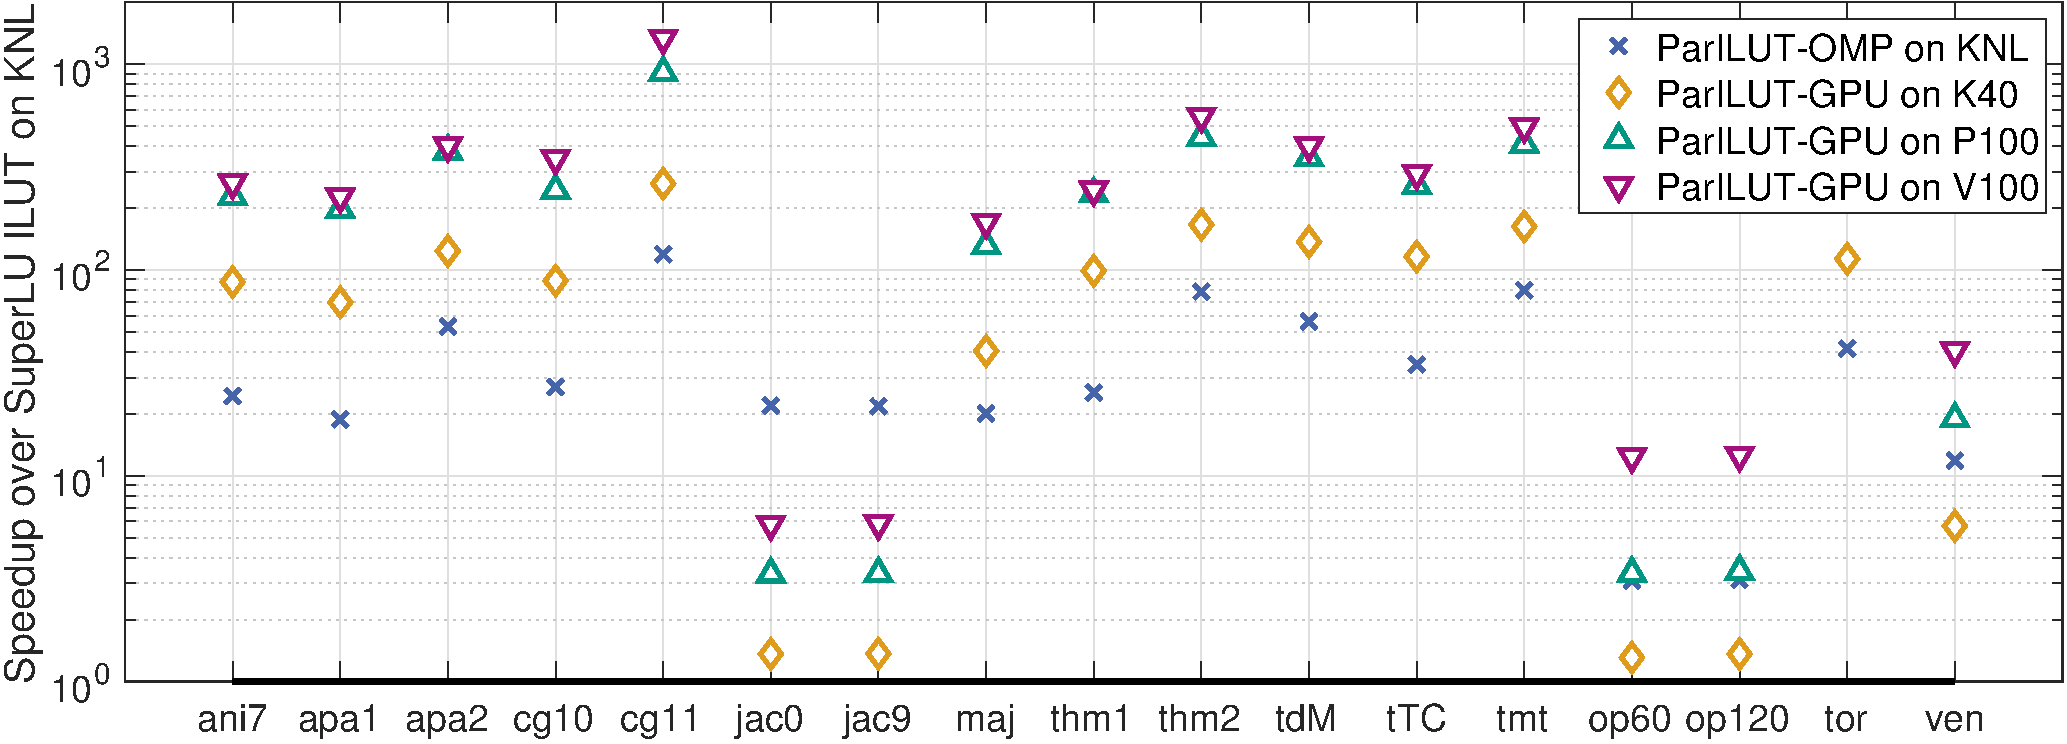
\includegraphics[width=5in]{projects/2.3.3-MathLibs/2.3.3.13-CLOVER/parilutspeedup}
	\caption{\label{fig:ParILUTperf}Speedup of the ParILUT over conventional 
	threshold-ILU generation on different manycore architectures. Test problems 
	are taken from the Suite Sparse Matrix Collection.}
\end{figure}


\paragraph{Next Steps}


Our next efforts are:
\begin{enumerate}
	\item \textbf{Low-synchronous orthogonalization:} The success of 
	communication-avoiding Krylov methods motivates to push the synchronization 
	limits further by deploying low-synchronous orthogonalization methods.
        (Collaboration with the ExaWind team at NREL.)
	\item \textbf{Parallel incomplete factorization preconditioner 
	application:} With the advances in the parallel incomplete factorization
	preconditioner generation, the focus increasingly turns to the efficient 
	preconditioner application. We enhance the concept of sparse approximate 
	inverse approximation for incomplete factorization preconditioners, and 
	extend the scope to novel hardware architectures featuring attractive 
	performance in the low-precision regimes.
%	\item \textbf{Get-set usage of software-defined events:} Together with the 
%	Exa-PAPI team, deployed software-defined events (SDE) in the Ginkgo sparse 
%	linear algebra library. These provide the user with access to 
%	domain-specific events like, e.g., preconditioner invocations, 
%	synchronizations, precision format changes. With building blocks differing 
%	in the resource usage, we investigate the possibility of instant power and 
%%	frequency scaling for reducing the power and energy footprint.
%	\item \textbf{Graph analytics kernels:} Preconditioning techniques like 
%	block Jacobi have a strong need for efficient and low-overhead graph 
%	analytics tools identifying strongly-connected components. We deploy GPU 
%	kernels providing this functionality while introducing only negligible 
%	overhead to the preconditioner generation.
	\item \textbf{Multiprecision sparse matrix formats:} Operations with sparse 
	matrices are memory-bound on virtually all architectures. We investigate 
	how splitting the matrix int several operators stored in value-optimized 
	less complex floating point precision formats can help improving
	performance.
	\item \textbf{Polynomial preconditioners:} The communication cost of 
	numerical preconditions is high. In particular for communication-avoiding 
	pipelined Krylov methods, the synchronization necessary by standard 
	preconditioning can become a bottleneck. We will deliver a new
        polynomial preconditioner in Trilinos (Belos) and investigate their effectiveness 
	for ECP applications.
\end{enumerate}
